\author{Gilles Hennenfent\/\footnotemark[1] and Sergey Fomel\/\footnotemark[2]}
\title{Madagascar for reproducible scientific publications tutorial}

\lefthead{Hennenfent \& Fomel}
\righthead{Reproducible scientific publications}

\newcommand{\rsf}{\textsf{Madagascar}\ }

\footnotetext[1]{Department of Earth \& Ocean Sciences, University of British Columbia at Vancouver. Email: ghennenfent@eos.ubc.ca}
\footnotetext[2]{Bureau of Economic Geology, University of Texas at Austin. Email: sergey.fomel@beg.utexas.edu}


\maketitle

\begin{abstract}
   xxx
\end{abstract}

\section{Introduction}

\rsf (formerly known as \textsf{RSF}) is an open-source software
package for reproducible geophysical data processing and computational
experiments. Its mission is to provide a simple yet powerful
environment and technology transfer tool for researchers working with
digital image and data processing. The technology developed using the
\rsf package is transferred in the form of recorded processing flows,
which become documented "computational recipes" to be verified,
exchanged, and modified by the entire \rsf community.

\subsection{Structure of a Madagascar reproducible document}

\rsf papers typically contain reproducible results from different
processing flows. Each of these flows is a sequence of processing
steps done using either \rsf command line programs or some other
software packages.

\begin{figure}[h]
\begin{center}
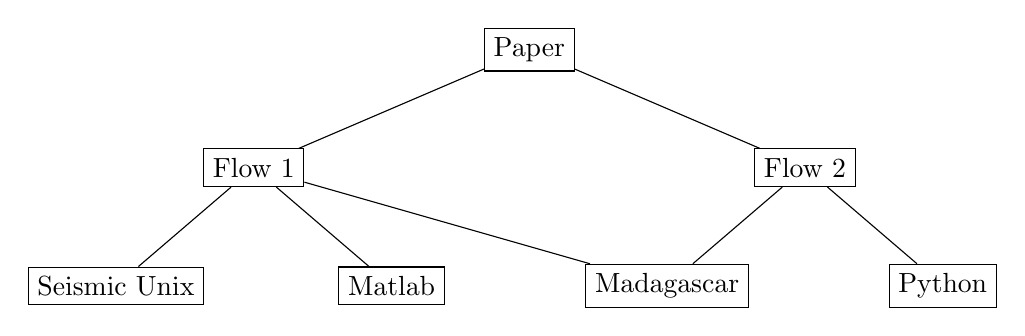
\begin{tikzpicture}
\tikzstyle{every node}=[rotate=0,draw]
\tikzstyle{level 1}=[sibling distance=70mm]
\tikzstyle{level 2}=[sibling distance=35mm]
\node (paper) {Paper}
child {node (flow 1) {Flow 1}
  child{node (su) {Seismic Unix}}
  child{node (matlab) {Matlab}}
}
child {node (flow 2) {Flow 2}
  child{node (rsf) {Madagascar}}
  child{node (python) {Python}}
};
\draw (flow 1) -- (rsf); 
\end{tikzpicture}

\end{center}
\caption{Structure of a \rsf reproducible paper}\label{fig:struct}
\end{figure}

\subsection{How to read this tutorial}


\subsection{Getting help}

Should you encounter a problem while working on your \rsf reproducible
document, please do the following:

\begin{itemize}
\item Read (again) this tutorial, at least the part that has to do
  with your problem.
\item If that does not solve the problem, try having a look at the
  \rsf user mailing list
  (\url{https://lists.sourceforge.net/lists/listinfo/rsf-user}) and
  \rsf webpage (\url{http://rsf.sourceforge.net/}). Perhaps someone
  has already reported a similar problem and someone has found a
  solution.
\item If you find out your problem was not addressed yet, mail it to
  the \rsf user mailing list. Someone will likely be able to help you
  in a timely fashion.
\end{itemize}

\section{Writing a reproducible scientific publications}
\subsection{SCons for processing flows}

Example of how to integrate Matlab, (Mathematica,) and Python would be
nice.

\subsection{\LaTeX\ document}
\subsubsection{SConstruct file}
Show how to Fetch non-repro figures.

\subsection{Website}

Construct a website from the \LaTeX\ document.

%%% Local Variables: 
%%% mode: latex
%%% TeX-master: t
%%% End: 
